\section{Background}
\label{sec:background}

\begin{figure}[t]
  \centering 
  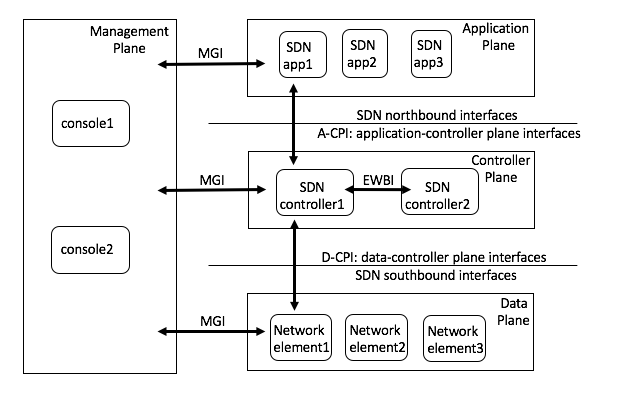
\includegraphics[width=3.3in]{img/sdn-arch.png} 
  \caption{SDN Architecture} 
  \label{fig:sdn-arch} 
\end{figure}

In this section, we first introduce the architecture and operation of
Software-Defined Networking (SDN). Next we give an overview of network 
reconnaissance, its utility to attackers, and the impact of successful
reconnaissance on an enterprise network's security. Finally  we discuss
how the architecture of SDN enables an adversary to perform reconnaissance 
in ways that were not feasible in traditional networks. 

\subsection{Software-Defined Networking}
SDN decouples the data plane of a network from the control plane
enabling  dynamic configuration and management of network devices through
programmable SDN applications that run on a network controller. The SDN
architecture can be divided into 4 different planes, which serve distinct
purposes and have their own defined functions. These planes contain one
or more entities or components working independently or together to
perform the tasks of a given plane. Communication between the planes is
made possible through various interfaces via open APIs and protocols. 

\subsubsection{Planes/layers identified in SDN}

We now describe the components and functions for three of the four 
different planes, which are relevant to this work. 

\myparagraph{Data plane} The data plane is comprised of a set of one or
more network elements (switches etc.) each of which contains a set of
traffic forwarding or traffic processing resources. The forwarding 
rules present on the switches are stored in flow tables as flow-entries 
that are set by the SDN controller. The data plane incorporates the 
resources that deal directly with customer traffic and some supporting
resources to ensure proper virtualization, connectivity, security, 
availability, and quality.
		
\myparagraph{Controller plane} The controller plane is comprised of a
set of SDN controllers that have exclusive control over a set of 
resources that are exposed by one or more network elements in the data
plane. The major role of an SDN controller is to execute requests of 
the SDN applications it supports and keep applications isolated from 
each other. Since a network may have more than one SDN controller, a
controller may communicate with peer controllers, subordinate 
controllers, or non-SDN environments, to carry out tasks on behalf of
applications.
	
\myparagraph{Application plane} The application plane is comprised of
one or more applications, each of which has exclusive control of a set
of resources exposed by one or more SDN controllers.  Several
applications can be operational at the same time performing various
different tasks and can alter the state of network resources or alter
the behavior of the data plane via the controller plane. An application
may invoke or collaborate with other applications and can also act as an
SDN controller in its own right.

\subsubsection{Interfaces identified in SDN}

To enable smooth communication between the planes and their underlying
components, there are four interfaces present in the SDN architecture. 
Here we describe just two of the four, which are relevant to this work.

\myparagraph{Northbound Interfaces (NBI)} The northbound interface 
exists between the controller plane and the application plane and 
enables communication between them. Several different applications 
can be operational in the application plane and can communicate with
the controllers using an exposed API. The controllers also respond to 
applications' requests and pass on information, events etc. to the 
applications using this interface.
	
\myparagraph{Southbound Interfaces (SBI)} The southbound interface 
exists between the controller plane and the data plane and enables
communication between the controllers and the network devices or
elements. The communication across this interface uses an open standard
protocol, such as the OpenFlow protocol. The controllers as well as the
network devices both the support this messaging protocol. The most 
common communication across this interface are control messages sent by
the controller to alter the behavior of the underlying network and
notifications from the network devices when they come online. 

Whenever a new flow is encountered by a switch, it first looks at its
flow table to check for a flow entry matching the given flow. If such a 
match is found, the switch applies the action stored in flow table for
the matching flow entry. If no match is found, the switch holds the 
packet in a buffer and sends the header information to the controller 
in the form of a \textit{packet\_in} message. This message transfer 
between the data plane and the control plane generally happens via 
OpenFlow~\cite{specification2015v151} protocol, which is a widely
popular SDN messaging protocol. Along with the packet header, the 
packet\_in message contains information about the physical port on the
switch the packet was received on. The controller has one or more SDN
applications registered with it that run in the application plane and
register event listeners for certain messages from the data plane, such
as packet\_in messages. As soon as the controller receives the 
packet\_in message, the controller fires a packet\_in event and the
applications registered for the corresponding handler are notified. The
applications then extract the flow information and perform certain logic
to decide the action to be done to the flow the packet belongs to. This
information is then passed to the controller from the applications by 
using the NBI. Finally, the controller sends down control messages to 
the switch in the data plane instructing what should be done to the 
flow by using the SBI. 

\subsection{Network Reconnaissance}
Before carrying out a major attack against a network, the attackers
generally attempt to gather as much information as possible. Most
importantly, they are focused on learning about the resources available,
their weaknesses and vulnerabilities, which resources are high value
targets, and what existing defense mechanisms are in the network and how 
they are distributed. This intelligence gathering phase is known as 
network reconnaissance. The attacker can use various methods such as 
surveillance, eavesdropping on and intercepting communications, and 
launching probes to gather information about the computer systems, 
policies, and other resources. Network reconnaissance either falls into
one of two categories:

\begin{figure}[t] 
  \centering 
  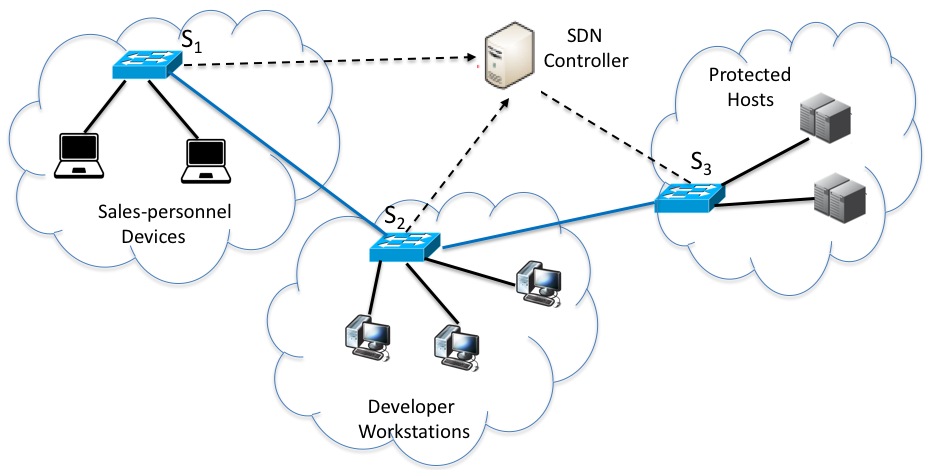
\includegraphics[width=3.3in]{img/topo.png} 
  \caption{A subset of Typical Enterprise SDN Deployment} 
  \label{fig:topo} 
\end{figure}

\myparagraph{Passive Network Reconnaissance} In this type of
reconnaissance, usually the adversary already establishes a foothold at
a very strong vantage point. For example, a strong vantage point in a 
network is at core switch. A core switch ties the network together,
seeing a lot of flows crossing its boundaries. An adversary controlling
one or more such switches can learn a lot about the topology of network, 
placement of security middleboxes, policies regarding communication 
between hosts, etc. by just passively observing the traffic passing 
through the switch. Therefore they can learn a lot without the need to 
perform any extra actions, and if and when required, may exfiltrate the 
gathered intelligence out of the network. Since the attacker does not 
perform any suspicious actions, attacks falling into passive
reconnaissance are very hard to detect in a network.

\myparagraph{Active Network Reconnaissance} In this type of
reconnaissance, an adversary controls a less advantageous vantage 
points, which gives only a local view of the network. Passively 
observing flows from this vantage point prevents an adversary from
learning about the entire network as only a small subset of flows are
observable. Therefore, the adversary uses specially crafted network
packets called probes to learn about other parts of the network.
Adversaries subtly send probes at low frequencies to avoid triggering a
defense mechanism using thresholds to identify anomalies in the network. 

Adversaries aim to learn the following information while performing
network reconnaissance:

\begin{itemize}
  \item{The topology of the network, including the locations of sensitive
  resources and security middleboxes.}
  \item{Active hosts accessible to external networks.}
  \item{The services and applications running in the network and any 
  vulnerabilities these services and applications may have that
  can be exploited to gain unauthorized access.}
\end{itemize}

In traditional networks, network reconnaissance using active probes has
been done by network port scanning or by directly interacting with other
hosts and devices on the network. Some of the techniques used for active
probing of a network include making use of mechanisms such as the TCP
handshake to judge a host's liveness, fingerprinting the protocol stack
to try to figure out the operating system the host is running, probing
DNS servers, and grabbing service banners volunteering information 
about the host.

The advent and popularization of SDN can lead adversaries to look for
new ways of network reconnaissance and different vantage points that
were not available or difficult to perform in a traditional network.

\myparagraph{Typical Enterprise Network (SDN)} Figure~\ref{fig:topo}
shows a subset of a typical enterprise network, comprised of several
different categories of hosts that perform different tasks, or are 
owned by employees performing different types of tasks. Generally, these
categories include developer workstations, sales and marketing devices,
HR owned laptops, and other highly sensitive resources such as Git 
servers, database servers, DNS servers, etc. Enterprises generally keep
these different categories of hosts in separate subnets for easy 
management and separation. In each subnet there are one or more subnet 
switches and the entire network has one or more SDN controllers
depending on the number of hosts. In such a setup, if the developer 
subnet switch is compromised by adversary, they would ideally want to 
learn more about the network before performing more serious attacks. 
They might check if hosts in the sales subnet have connectivity with a 
protected resource they are targeting. This information is useful for a 
number of reasons. For example, if sales devices are running an OS that 
is different than the OS running on the developer workstations and the
sales devices have an unpatched vulnerability, using the sales device to
access the protected resource may be easier than using the developer
workstation. This scenario illustrates the need to detect network
reconnaissance in a network, the next section explicitly states all
assumptions about the adversary and the network environment we consider
in this work.
